\documentclass[journal, a4paper]{IEEEtran}

\usepackage{graphicx}   
%\usepackage{subfigure}
\usepackage{url}        
\usepackage{amsmath}    
% Some useful/example abbreviations for writing math
\newcommand{\argmax}{\operatornamewithlimits{argmax}}
\newcommand{\argmin}{\operatornamewithlimits{argmin}}
\newcommand{\x}{\mathbf{x}}
\newcommand{\y}{\mathbf{y}}
\newcommand{\ypred}{\mathbf{\hat y}}

% Start of added stuff by lukas
%\newtheorem{defi}{Definition}[section]
% Packages
\usepackage{mathtools}
\usepackage{amsmath}
\usepackage{amssymb}
\usepackage{amsthm}
% Theorems and definitions
\theoremstyle{plain}
\newtheorem{thm}{Theorem}
\theoremstyle{definition}
\newtheorem{defn}[thm]{Definition}
% Algorithm description
\usepackage{algorithm}
\usepackage[noend]{algpseudocode}
\makeatletter
\def\BState{\State\hskip-\ALG@thistlm}
\makeatother
% Figures
\usepackage{svg}
% End of added stuff by lukas

\begin{document}

% Define document title, do NOT write author names
\title{The Title of your Report}
\author{Anonymous Authors}
\maketitle

% Write abstract here
\begin{abstract}
	A short summary of your project. You should change also the title, but do \emph{not} enter any author names or anything that unnecessarily identifies any of the authors. It is suggested you use a similar structure (sections, etc.) as demonstrated in this document, but you can make the section headings more descriptive if you wish. Of course \emph{you should delete all the text in this template and write your own}! -- this text simply provides detailed instructions/hints on how to proceed.

\end{abstract}

% Each section begins with a \section{title} command
\section{Introduction}

%Describe what you did. Provide access to your anonymized code\footnote{Our code is available here: \url{http://anonymouslinktoyourcode.zip}}.

%Note that results should be reproducible using the technologies from the labs (i.e., Python, and selecting among Scikit-Learn, OpenAI Gym, TensorFlow, PyGame, \ldots).

%Do not change the formatting (columns, margins, etc). Hint: shared tools like \texttt{http://sharelatex.com/} and \texttt{http://overleaf.com/} are great tools for collaborating on a multi-author report in latex. If you wish to use Word, base it on the IEEE template\footnote{\url{https://www.ieee.org/publications_standards/publications/conferences/2014_04_msw_a4_format.doc}} and convert to \texttt{pdf} for submission. 

In the following paper we implement three different reinforcement learning agents and evaluate their performance within a supply chain environment. All the code used to create the results presented in this paper can be found here \footnote{Our code is available here:\url{http://anonymouslinktoyourcode.zip}}. \newline
The supply chain optimization environment represents a problem faced by companies whose supply chain consists of a factory and multiple warehouses (so called hub-and-spoke networks as described by \cite{MFL}). The main decision that needs to be made in these settings is how many products should be produced in the factory and how much stock should be build up in the warehouses. Seasonal demand can further complicate the decision problem since it might require the companies to start building up stock early so that high demands in the future can be satisfied (e.g. think about christmas where the stock of eggnog needs to be build up during november and december to be able to satisfy the high demand levels during the holidays). This requirement for mid- to long-term planning indicates that the problem can be formulated as a multi-step decision problem and further exhibits a weak signal because the reward for an early build-up of stock will only be realized in the future when the actual demand reaches its maximum. \newline
Even for small supply chain networks we find that due to the curses of dimensionality, as described by \cite{PowellADP}, the state- and action-spaces of the respective decision problems become unfeasebly large. Therefore we turn to function-approximation and policy-search methods of reinforcement learning that are less affected by these problems. In our case we chose approximate SARSA and the REINFORCE algorithm as a basis for the agents.
\section{Background and Related Work}
%Elaborate (in your own words) the background material required to understand your work. It should cover a subset of the topics touched upon in the course. You are encouraged to cite topics in lectures, e.g., structured output prediction in \cite{LectureSOP}, book chapters, e.g., Chapter 9 from \cite{Barber}, or articles from the literature, e.g., \cite{Astar,DeepMindSC2}. Basically, you should prepare the reader to understand what you are about to present in the following sections. Eq.~\eqref{eq:MAP} shows a random equation.
%\begin{equation}
%	\label{eq:MAP}
	% Note the example \newcommand s defined above which make it faster to write latex math
%	\ypred = \argmax_{\y \in \{0,1\}} p(\y|\x)
%\end{equation}
The supply chain optimization problem presented in this paper will be modeled as a markov decision process (MDP). Furthermore we rely on the approximate SARSA and REINFORCE algorithms to design agents capable of finding a good strategy to navigate within the environment. \newline
MDPs are multi-step stochastic decision problems that rely on the markov property which implies that the transition probability $P(s_{n+1} \ | \  s_n)$ between two states $s_{n+1}$ and $s_n$ only relies on the current state $s_n$. We describe the MDP similar to \cite{Moritz} and \cite{PowellADP} as an eight-tuple $(S, D, A, \mathcal{X}, T, Q, r, \gamma)$ consisting of a state-space $S$, a random environment process $D$, an action space $A$, a set of feasible actions $\mathcal{X}$, a transition function $T$, transition probabilities $Q$, a one-step reward function $r$ and some discount factor $\gamma$. \newline
The designed agents are based on the blueprints for the approximate SARSA and REINFORCE algorithm from \cite{LectureDRL}. We compare the performance of these reinforcement learning algorithms with an agent that acts according to a fixed heuristic based on the $(\varsigma, Q)$-Policy \footnote{In the literature this policy is usually called $(\varsigma, Q)$-Policy. We chose a slightly different name to avoid notation conflicts in our model description.} as described by \cite{sQ}. $(\varsigma, Q)$-Policies induce a simple replenishment strategy where the stock of a warehouse will be replenished by some amount $Q$ as soon as it falls under a threshold $\varsigma$. A basic visualization of the $(\varsigma, Q)$-Policy is depicted in Figure~\ref{sQ}.
\begin{figure}[h]
	\centering
	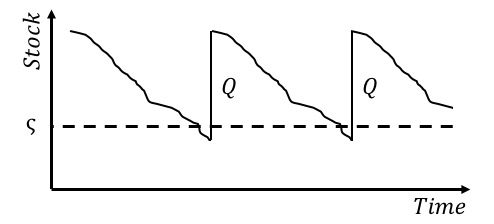
\includegraphics[width=0.8\columnwidth]{sQ.jpg}
	\caption{\label{sQ} Schematic visualization of a $(\varsigma, Q)$-Policy for a single warehouse.}
\end{figure}
\newline
Furthermore we use several different stepsize formulars from \cite{PowellADP} that are used to update some of the agents parameters such as the learning rate $\alpha$. The idea of specific stepsize rules is to allow the agent to go through a longer learning phase in the beginning with higher learning rates and then converge in the long term to stepsizes close to $0$. %This behavior can be seen in \ref{fig:stc_stepsize}. that shows the learning rates generated from 
Among others we use a so called search-then-converge stepsize rule as presented in \cite{PowellADP} where the learning rate in the $n^{th}$ iteration is calculated by
\begin{equation}
\label{eq:stc}
	\alpha_n = \alpha_0 \frac{\frac{b}{n} + a}{ \frac{b}{n} + a + n^{\beta}}
\end{equation}
with some parameters $\alpha_0, b, a$ and $\beta$ that can be set by the user based on the required behavior of the stepsize.
%\begin{figure}[h]
%	\label{fig:stc_stepsize}
%	\centering
%	\includegraphics[width=0.6\columnwidth]{STC.png}
%	\caption{\label{stc} Learning rates of the search then converge stepsize for $24.000$ iterations.}
%\end{figure}
\section{The Environment}
We will model the environment as a MDP that we regard over an infinite number of periods $t = 0, 1, ...$ . The environment consists of one factory (indexed by $0$) and up to $k \in \mathbb{N}$ warehouses (indexed by $j=1,...,k$) where in each period it needs to be decided how many units of a product (e.g. butter) should be produced and how many should be shipped to the individual warehouses. A representation of a network with 5 warehouses is depicted in Figure~\ref{model_example}. 
\begin{figure}[h]
	\centering
	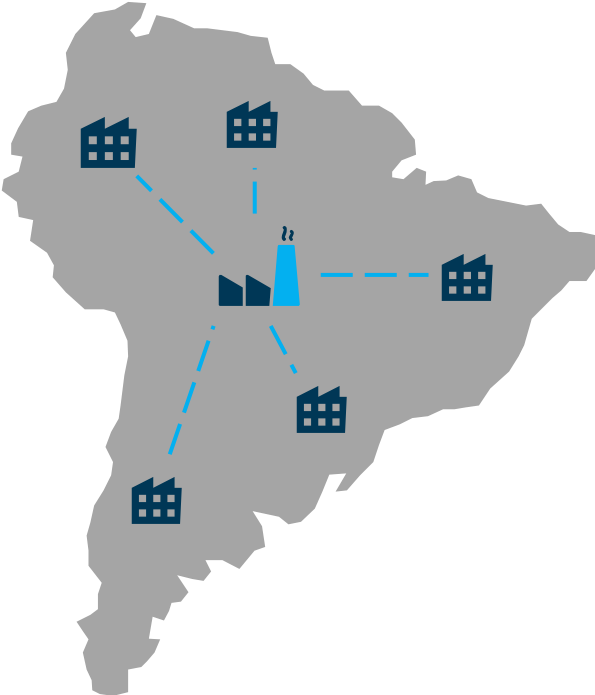
\includegraphics[width=0.4\columnwidth]{model.png}
	\caption{\label{model_example}Example of a supply chain network with $k=5$ warehouses ($s_1, .., s_5$) and the factory ($s_0$).}
\end{figure}
The state space consists of $k+1$ elements describing the current stock levels of the factory and the warehouses ($s_j, j=0,...,k$), where each stock level is limited by some capacity $c_j \in \mathbb{N}$. Note that this implies that the factory itself can also build up stock. Furthermore we assume an environment process with states $d \in D \in \{0,..., d_{max}\}^k, d_{max} \in \mathbb{N}$ describing the (stochastic) demand $d_j$ at each warehouse with transition probabilities $q_d(d')$ that are unknown by the agent. We assume a discretized version of a sinus-function and some shocks $\epsilon$ where the demand follows a model 
\begin{equation}
	\begin{split}
		d_{i,t} = &\left\lceil \frac{d_{max}}{2} \sin\left( \frac{2 \pi (t + 2i) }{12}\right) + \frac{d_{max}}{2} + \epsilon_{i,t} \right\rceil
	\end{split}
\end{equation}
with $\left\lceil \cdot \right\rceil$ the ceiling function and $P(\epsilon_{i,t}=0) = P(\epsilon_{i,t}=1) = 0.5$. We will include $d_{last}, d_{hist} \in D$ in our state space where for some time $t$ we have the tuple $\tilde{s} = (s, d_{last}, d_{hist}) \in \tilde{S} \coloneqq S \times D^2$ with $s = s_t$, $d_{last} = d_{t-1}$ and $d_{hist} = d_{t-2}$. Note that this implies that the demand $d_t$ of period $t$ is not observed by the agent. This means, that the demand in a period $t$ will be realized after observing the stock levels $s_t$ and can only be observed in the next period $t+1$.
%since the demand $d_{i, t}$ is correlated with the demand $d_{i, t+1}$. Note that each tupel $(s, d, d_{hist})$ at some point in time $t + 1$ consists of the current state, the last observed demand and the  \left($(s_{t+1}, d_t, d_{t-1})$\right). 
The reason we add the old demands to the state space is to allow the agent to have a simple understanding of the demand history to be able to gather a basic understanding of the demands movement. In each period the agent can now set the factories production level for the next period $a_0 \in \{0,.., \rho_{max}\}$ (with a maximum production of $\rho_{max} \in \mathbb{N}$) aswell as the number of products shipped to each location $a_j \in \mathbb{N}^k$ that is naturally limited by the current storage level in the factory ($\sum_{j=1}^{k}a_j \leq s_0$). Based on this information and the demand $d$ we can now describe the state transitions $(\tilde{s}, d, a) \rightarrow T(\tilde{s},d,a)$ by
\begin{equation}
\label{eq:transition_function}
	\begin{split}
		T(\tilde{s}, d, a) \coloneqq (&\min\{s_0 + a_0 - \sum_{j=1}^{k}a_j, c_0 \}, \\
		&\min\{s_1 + a_1 - d_1, c_1 \}, \\
		&\ ... \\
		&\min\{s_k + a_k - d_k, c_k \}, \\
		&d, \\
		&d_{last}).
\end{split}
\end{equation}
%\begin{equation}
%	\begin{split}
%		s_0' = &\min\{s_0 + a_0 - \sum_{j=1}^{k}a_j \}, \\
%		s_j' = &\min\{s_j + a_j - d_j\}, \ j=1,...,k.
%	\end{split}
%	\end{equation}
The reward within each period consists of the revenue from sold products at a fix price $p$ less production costs $\kappa_{pr}a_0$, storage costs $\sum_{j=0}^{k}\kappa_{st,j} \max\{s_j, 0\}$, penalty costs $\kappa_{pe} \sum_{j=1}^{k}\min\{s_j,0\}$ and transportation costs $\sum_{j=1}^{k} \kappa_{tr, j} \left\lceil a_j / \zeta_j \right\rceil$. We let $p, \kappa_{pr}, \kappa_{pe}, \kappa_{st, j}, \kappa_{tr,j} \in \mathbb{R}_+$ and $\zeta_j \in \mathbb{N}$. We can now define the one-step reward function by
\begin{equation}
\label{eq:one_step_reward}
	\begin{split}
		r(\tilde{s}, d, a) \coloneqq &p \sum_{j=1}^{k}d_i - \kappa_{pr} a_0 - \sum_{j=0}^{k} \kappa_{st, j} \max\{s_j, 0\} \\ 
		&+\kappa_{pe} \sum_{j=1}^{k}\min\{s_j, 0\} - \sum_{j=1}^{k} \kappa_{tr, j} \left\lceil \frac{a_j}{\zeta_j} \right\rceil.
	\end{split}
\end{equation}
Furthermore we chose a discounting factor $\gamma \in (0,1)$ that can be interpreted e.g. as a result of inflation. \newline Based on this model description we can now formulate the task as an infinite horizon markov decision process that is subject to a varying environment. Thereby we receive the tuple $(\tilde{S}, D, A, \mathcal{X}, T, Q, r, \gamma)$ with
\begin{defn} \label{def:modell} \
	\begin{itemize}
		\item[1.] $\tilde{S}  \times D \coloneqq \prod\limits_{j=0}^{k} \{s_j \in \mathbb{Z} \ | \ s_j \leq c_j\} \times D^3, c_j \in \mathbb{N}$ the state space consisting of elements $(\tilde{s}, d) = ((s, d_{last}, d_{hist}), d)$;
		\item[2.] $ A \coloneqq  \{0, ..., \rho_{max} \} \times \mathbb{N}_0^k$ the action space consisting of elements $a = (a_0, ..., a_k)$;
		\item[3.] $ \mathcal{X} (\tilde{s}) \coloneqq \{0, ..., \rho_{max} \} \times \{a \in \mathbb{N}_0^k \ | \ \sum_{j=1}^{k}a_j \leq s_0  \}$, the set of all feasible actions in a state $\tilde{s}$ and $\mathcal{X} \coloneqq \{(\tilde{s}, d , a) \in \tilde{S} \times D \times A \ | \ a \in \mathcal{X} (\tilde{s})\}$;
		\item[4.] $ T: \tilde{S}  \times D \times A \rightarrow S$ the transition function defined by Eq.~\eqref{eq:transition_function};
%			\begin{equation*}
%				\begin{split}
%					T(s, d, a) \coloneqq &(\min\{s_0 + a_0 - \sum_{j=1}^{k}a_j, c_0 \}, \\
%					&\min\{s_1 + a_1 - d_1, c_1 \}, \\
%					&\ ... \\
%					&\min\{s_k + a_k - d_k, c_k \});
%				\end{split}
%			\end{equation*}
		\item[5.] $ Q: \mathcal{X} \times \tilde{S} \times D \rightarrow [0,1]  $ the transition probabilities with $Q(\tilde{s}', d'\ |\ \tilde{s}, d, a) \coloneqq q_d(d')$ for $\tilde{s}' = T(\tilde{s}, d, a)$ and $0$ otherwise;
		\item[6.] $ r: \tilde{S} \times D \times A \rightarrow \mathbb{R} $ the one-step reward function as described in Eq.~\eqref{eq:one_step_reward};
%			\begin{equation*}
%				\begin{split}
%					r(s, d, a) \coloneqq &p \sum_{j=1}^{k}d_i - \kappa_{pr} a_0 - \sum_{j=0}^{k} \kappa_{st, j} \max\{s_j, 0\} \\ 
%					&-\kappa_{pe} \sum_{j=1}^{k}\min\{s_j, 0\} - \sum_{j=1}^{k} \kappa_{tr, j} \left\lceil \frac{a_j}{\zeta_j} \right\rceil;
%				\end{split}
%			\end{equation*}
		\item[7.] $\gamma \in (0, 1) $ the discounting factor.
	\end{itemize}
\end{defn}
For the calculation of the expected discounted revenue for each tuple $(\tilde{s}, d)$ we obtain the value function $V$ with\\
\begin{equation}
	\label{eq:ValueFunction}
	\begin{split}
		V(\tilde{s},d) = &\max_{a \in \mathcal{X} (\tilde{s})} \{ r(\tilde{s}, d, a)  \\
		&+ \gamma \sum_{d' \in D} q_d(d') V(T(\tilde{s}, d, a), d') \}, \\ 
		&\tilde{s} \in \tilde{S}, d \in D. 
	\end{split}
\end{equation}
\section{The Agent}
%The agent you designed for your environment. Justify your choice and design and explain briefly how you implemented/configured it. Naturally, if you took a %ready-made environment, you should invert relatively much more effort into this section than the previous one.
In this paper we evaluate the performance of three agents based on different algorithms: a heuristic based on the $(\varsigma, Q)$-Policy that we use as the baseline for performance evaluation, an approximate SARSA algorithm and an implementation of the REINFORCE algorithm. \newline
\textbf{The $(\varsigma, Q)$-Policy} based agent is not smart in the way that it does not learn over time. Due to the popularity of the $(\varsigma, Q)$-Policy in practice we use it as a baseline for performance evaluation of the other agents. In the heuristic we iterate over $s_1, ..., s_k$ and replenish the respective warehouses by some amount $a_i = Q_i$ if the current stock is below a level $\varsigma_i$ and there is still stock left in the factory $s_0$. At the end we set the production level for the next period to $Q_0$ if $s_0 - \sum_{i=1}^{k}a_i < \varsigma_0$ and $0$ otherwise. The thresholds $\varsigma$ and replenishment levels $Q$ need to be set by the user when initializing the agent.
\newline
\textbf{Approximate SARSA} uses a linear approximation $Q_{\theta}(\tilde{s}, a) = \theta^T \phi(\tilde{s},a)$ of the Q-function. We chose this method as it solves the problem of exponentially growing state- and action- spaces that is likely to occur in multidimensional environments. Furthermore it allows us to use our knowledge of the environment (especially the structure of the reward function $r(\tilde{s}, d, a)$) to design $\phi(\tilde{s}, a)$ such that it preserves some of the MDPs structure. The algorithm is implemented as depicted in \cite{LectureDRL} where we use an $\epsilon$-Greedy strategy to select the action and a search-then-converge stepsize rule to update the learning rate $\alpha$ and the probability of chosing a random action $\epsilon$ as defined in~\eqref{eq:transition_function}. \newline
One of the crucial tasks when designing the approximate SARSA agent is the model for $\phi: \tilde{S} \times A \rightarrow \mathbb{R}^p, p \in \mathbb{N}$. This can be understood similar to feature engineering where we use some state $s$ and some action $a$ to compute $p$ features that should be capable of describing $Q(s,a)$. In our case we create over $15$ different types of features that can be binary as well as continuous. One of the main ideas is to get a rough estimate of the next demand and state by
\begin{equation}
	\begin{split}
		\hat{d}(\tilde{s})&= d_{last} + \left( d_{last} - d_{hist} \right) = 2d_{last} - d_{hist}, \\
		\hat{s}(\tilde{s}, a) &= T(\tilde{s}, \hat{d}(\tilde{s}), a)_{(d, d_{last})},
	\end{split}
\end{equation}
where $T(\cdot)_{(d, d_{last})}$ is the transition function excluding its last two elements. This way the agent can get a basic understanding of rewards and penalties associated with $\hat{s}$. Among others we use the expected penalty costs, the expected reward and the squared difference of the stock levels $s$ from their $25\%, 50\%$ and $75\% $ maximum capacity. Furthermore we include the respective rewards and costs for two scenarios where $\hat{d}^+=\hat{d}(\tilde{s}) + 1$ and $\hat{d}^-=\hat{d}(\tilde{s})  - 1$. While designing the agent we ended up with two different functions $\phi$ and $\phi^\prime$ that affect the agents behavior. Both functions have been tested and are included in our code. We encourage the reader to try out both. A full list of all features can be found in the appendix. \newline
%The underlying intuiton for the definition of $\phi$ is to value states $\tilde{s}$ based on an approximation of the individual storage levels, recent demands $(d_{last}, d_{hist})$ and the sales price $p$. We assume that the stock in each warehouse $s_1,..., s_k$ will be roughly equivalent to the current stock level minus the current demand (which is used as a proxy of the demand in the next step). For the factory $s_0$ we solely regard the current storage level but deduct the production cost $\kappa_{pr}$ from the sales price. Based on this intuition we can define $\phi: S \times D \times A \rightarrow \mathbb{R}^{k+1}$ by
%\begin{equation}
%	\label{eq:sarsa_phi}
%	\begin{split}
%	\phi(s, a) \coloneqq (&(s_0 + a_0)(p - \kappa_{pr}), \\
%	&(s_1 + a_1 - d_1)p, \\
%	&\ ... \\
%	&p (s_k + a_k - d_k)p ).
%	\end{split}
%\end{equation} 
When testing the approximate SARSA algorihm we found that for some environments the parameters $\theta$ would increase until computations became numerically unstable. To avoid this issue we restrict the temporal difference
\begin{equation}
	\delta_n = r(\tilde{s_n}, d_n, a_n) + \gamma \theta_n^T \phi(\tilde{s}_{n+1}, a_{n+1}) - \theta_n^T\phi(\tilde{s}_n, a_n)
\end{equation}
that is used to update $\theta_n$ within the intervall $[-1\mathrm{e}{100}, +1\mathrm{e}{100}]$. Furthermore we initialize the agent with a very small stepsize $\alpha$. 






\textbf{REINFORCE} is based on a parametrized policy for which the expected reward has to be maximized. We assume our policy to be parametrized as a softmax function for multiple actions. The softmax function assigns a probability for each action and thus behaves as a stochastic policy which can, however, converge to a deterministic one. 
We discretize the action space such that we only have three available actions per entity (for each warehouse and the factory). For a warehouse, for example, these possible actions are an order of  0,1 or 2 full trucks from the factory. For a given state, some actions might not be available. Since a projection of an unfeasible action to the closest feasible action is not possible in our environment, we used an alternative approach which only updates parameters for available actions. 
This leads to the following policy parametrization:
\begin{align}
    \label{simple_equation}
    p( a = a^{(k)}| s) = \pi_\Theta(a = a^{(k)},s) =
    \notag
    \\
     =\frac{e^{\Phi(s)^T w_{a^{(k)}}}\cdot f(a^{(k)}|s)}{\sum_{j=1}^{n_a} e^{\Phi(s)^T w_{a^{(j)}}}\cdot f(a^{(j)}|s)} 
     :=
     \sigma_k(s)
\end{align}
where 
\begin{equation}
   f(a^{(j)}|s) =
   \begin{cases}
     1 & \text{if $a^{(j)}$ is allowed in state s} \\
     0 & \text{otherwise} \\ 
   \end{cases}
\end{equation}
As we allow 3 different actions per entity, the number of possible actions is $n_a = 3^{(n_{stores}+1)}$. 
The feature map $\Phi(s): \mathbb{Z}^{n_{stores}+1} \rightarrow \mathbb{R}^{d}$ maps the state into a space of dimension d in which an optimal action is easily seperable from the other ones. We tried several different options for $\Phi(s)$ including first and second order terms and radial basis functions. 
The parameter matrix $\Theta$ is assembled in the following way:
\begin{equation}
	\Theta = \big(w_1|w_2|...|w_{n_a}\big) \in \mathbb{R}^{d \times n_a }
\end{equation}
where $w_i \in \mathbb{R}^{d}$ (including a bias). We initialized $\Theta$ to zeros in order to start with equal probabilities for each action.
\newline
\newline
A gradient ascent method is used to find the parameters that maximize the expected reward following this policy. The gradient for our parametrization evaluates to:
%	\nabla_{w_i}J(\Theta) = 
\begin{equation}
\notag
\nabla_{w_i} ln(\pi_\Theta(a^{(k)},s))D_t=
	\begin{cases}
     (1-\sigma_i(s)) \Phi(s)D_t  & \text{if $i = k$} \\
     -\sigma_i(s)\Phi(s)  D_t & \text{if $i \neq  k$} \\ 
    \end{cases}
\end{equation}
The full derivation for this gradient is shown in the Appendix.\newline
A key parameter for this algorithm is the learning rate which we left constant, but close to zero since a small learning rate allows a lot of exploration which is needed for all parameters to adapt. 



\section{Results and Discussion}



%This is one of the most important sections. You put your agent to the test in the environment, you show -- and most importantly -- you interpret the results.

\subsection{Performance of your Agent in your Environment}

%Show plots, graphs, tables (e.g., Table~\ref{a_table}), etc. You may wish to encourage readers to reproduce results for themselves, e.g., run \texttt{runDemo.py} in our source code. Show how your agent performs well, or, if it doesn't perform well, it is better to explain why (this is a result in itself!). In any case, you \emph{must} highlight the weaknesses of your agent as well as its strengths. \newline
%\begin{table}[h]
%	\caption{\label{a_table}This table is just an example.}
%	\centering
%	\begin{tabular}{lll}
%		\hline
%		\textbf{Environment config.} & \textbf{Standard SARSA} & \textbf{Our Improved Agent}  \\
%		\hline
%		Simulation 1        & 10             & 15 \\
%		Simulation 2        & 12             & 11 \\
%		\hline
%	\end{tabular}
%\end{table}


To test the algorithms, two main test were done. All of the tests were computed using 10000 episodes of 24 steps each in which our demand distributions make a whole cycle, allowing it to have the full seasonal demand.\newline
%%%%%%%%%%%%
%The first test with only the factory and one warehouse includes %production cost, a storage cost for the warehouse only, a %transportation cost, and a penalty cost for not delivering enough %products. A strategy for the agents to learn is that even though %the costs for production, storing and transportation give a %negative short-term reward, they are necessary to avoid huge %penalty costs in the future. Since the demand increases towards %the end of the year, the optimal strategy is to build up stock, %since production alone cannot satisfy this demand.
%%%%%%%%%%%%%%%
The first test is a simple test, having only the factory and one warehouse,  with no storage cost in the factory and small cost of production, transportation and storage in the warehouse. The objective of this test was to see if the agents can learn that even if producing, sending and storing is a bad decision in short term, because there is a penalty cost that accumulates for not sending the goods to the warehouse, the overall strategy should be to do it anyway.

%%%%%%%%%%
 But because there is a cost of production, the optimal strategy would be to not build as much as we can but to build enough to be able to satisfy the season of high demand but no more than that.
\begin{figure}[h]
	\centering
	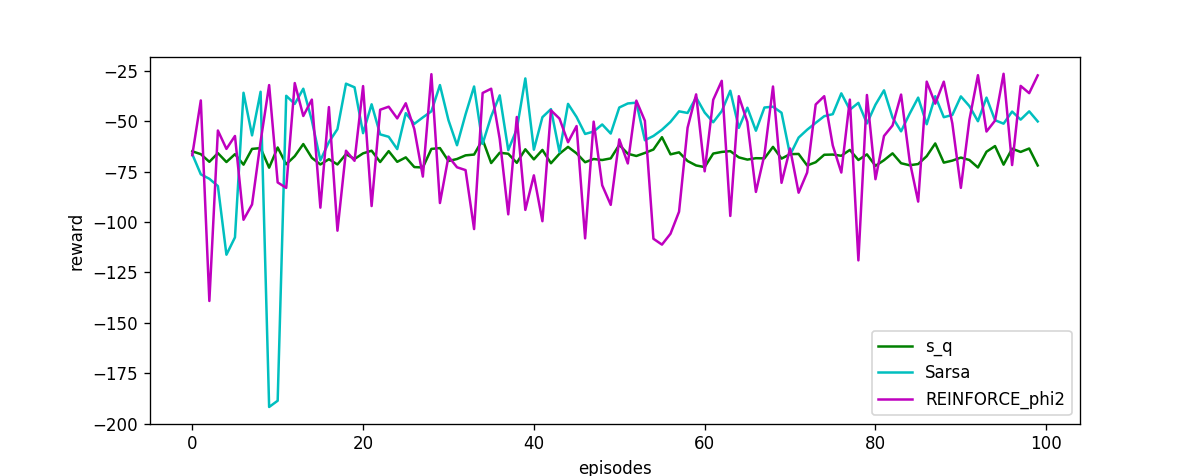
\includegraphics[width=0.8\columnwidth]{medium_2_env_rewards.png}
	\caption{\label{medium_2_env_rewards} Rewards over time for the three agents in the first test.}
\end{figure}
\newline
The graph seen in Figure 3 shows that both the approximate SARSA algorithm and the REINFORCE can learn this task, with the REINFORCE algorithm having slightly better results and with notable better results that the $(\varsigma, Q)$-Policy based agent, who sends and produces goods before they are needed and ends up getting a higher penalty. This shows that the basis of our environment can be learned by our agents even if they are only getting weak signals.\newline
The second test is a harder environment. In this environment the number of warehouses went up to 3, each with different properties. The first warehouse has a high storage and transportation cost, the second warehouse has no storage cost but high transportation cost and the third one no transportation nor storage cost. Furthermore, because of how the production and the demand are balanced there are not enough goods to satisfy all the demand, the agent need to learn everything he learned in the simple scenario but also to prioritize some warehouses before others.
\begin{figure}[h]
	\centering
	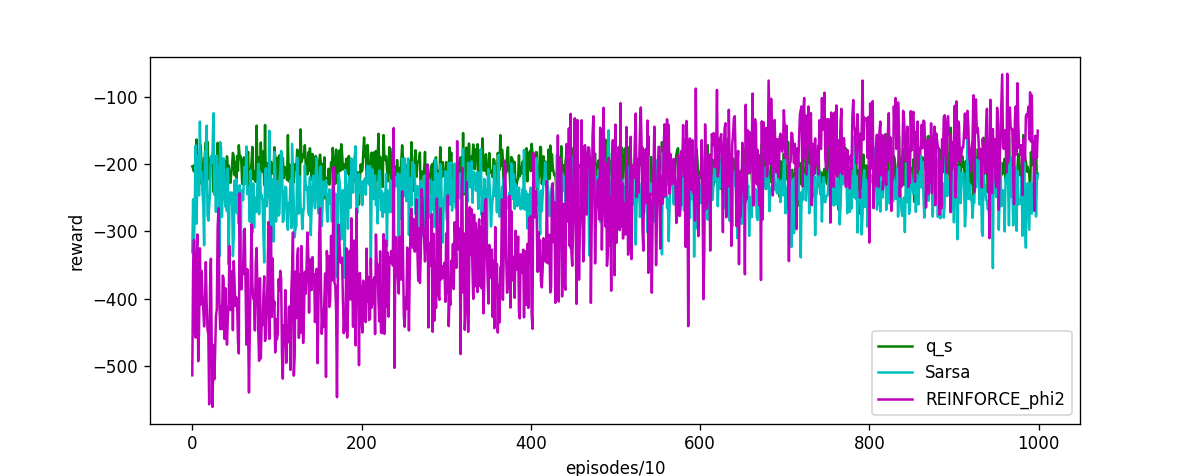
\includegraphics[width=0.8\columnwidth]{weird_2_env_rewards.png}
	\caption{\label{weird_2_env_rewards} Rewards over time for the three agents in the second test.}
\end{figure}
\begin{figure}[h]
	\centering
	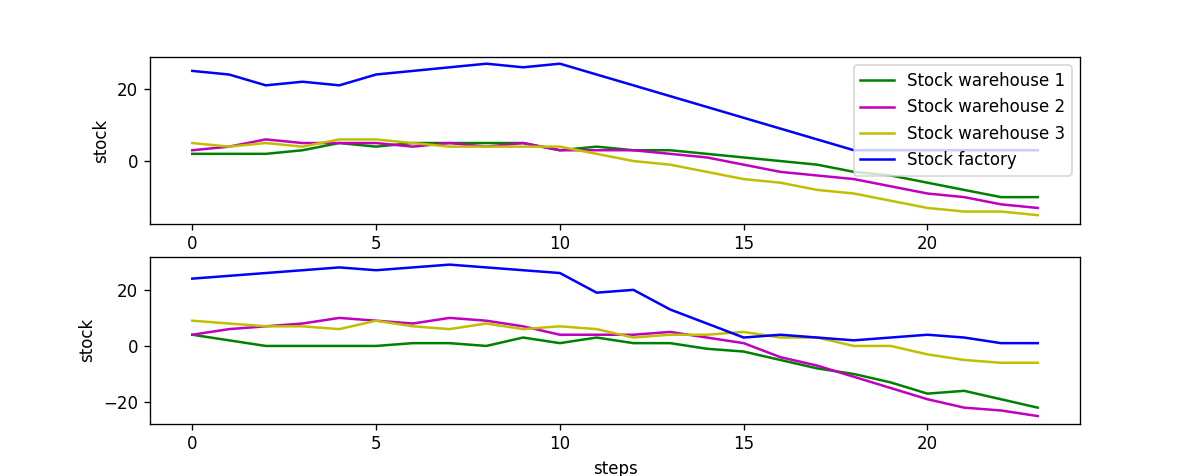
\includegraphics[width=0.8\columnwidth]{stocks_weird_2_env.png}
	\caption{\label{stocks_weird_2_env} Stocks for the $(\varsigma, Q)$-Policy based agent and the REINFORCE agent in the second test.}
\end{figure}
\newline
This second graphs seen in Figure 4 shows the $(\varsigma, Q)$-Policy based agent who begins with better results thanks to his simple solutions that allows him to produce a lot and send it to fill the stores one by one, but after all the training the REINFORCE algorithm manages to learn a better strategy. As shown in Figure 4, the storage levels in the differents stores for the $(\varsigma, Q)$-Policy strategy are pretty similar while on the REINFORCE we have the warehouse 1 who has at beginning almost zero stock due to its high storage cost, and when the demand is too high both warehouse 1 and 2 are forfeit to the store three, thanks to his zero cost of storage and transportation. \newline
The SARSA on the other hand does not manage to learn the right strategy, building less stock during the low demand and not prioritizing early the warehouse three. The main problem from the not learning of the SARSA is the difficulty to choose the right features and to allow the agent to learn what needs to be learn with this features. Here, we can’t just have a feature that is storage level due to the fact that having really high storage is bad but low is also bad. And because of how the value of each action in every state is calculated is a weight times the feature, he can either say “producing is bad” or “producing is good”. So a balance between the features needs to be reached, where the agent can say that producing is good unless there is too much. This balancing of feature is hard to learn and provoques bad results in too complicated scenarios. This might be solved with a different combination of features but for this particulars parameters none was found.\newline
The readers are encouraged to create their own scenarios in testing.py to see the different performances of the agents. To compare their performances or recreate the graphs seen in this paper graph\_creation.py needs to be run.

 


\subsection{Performance of your Agent in the ALife Environment}
%You deploy your agent in the ALife\footnote{\url{https://github.com/jmread/alife}} environment (a random screenshot shown in Figure~\ref{a_figure}). Does it work well? Why? Why not? Justify the adaptation you think is best.
%\begin{figure}[h]
%	\centering
%	
\includegraphics[width=0.8\columnwidth]{alife.png}
%	\caption{\label{a_figure}An example figure}
%\end{figure}
Our implementation of the approximate SARSA algorithm uses a very specific value function approximation that depends strongly on assumptions about the underlying environment. Since this environment has no structural similarity with the ALife\footnote{\url{https://github.com/jmread/alife}} environment it can not be used for testing. To adapt the algorithm to the ALife environment it would be necessary to create new features and design a different function $\phi$ to be used within the existing agent.
\newline
In general, the REINFORCE approach is very nicely applicable to the Alife environment as was shown in the lab. Allowing multiple possible actions can also be a reasonable extension. Our implementation, however, is not directly transferable, since we use additional information about which actions are possible which is not available in the Alife environment.
\section{Conclusion and Future Work}
The REINFORCE approach is certainly a viable option for this environment as it performs well in each scenario. Of course, the algorithm does have some downsides. As a gradient ascend algorithm it can easily get stuck in local optima which can easily arise in this possibly highly non-convex setting. 
Additional drawbacks come from the softmax parametrization which 
requires parameters for each action. This requires a lot of training and can lead to difficulties for actions that are rarely feasible. Moreover, the actions to replenish 0, 1 or 2 trucks are treated as completely separate, dropping the possibility to make use of their ordering. Another parametrization that would make use of this order would be e.g. a Gaussian setting. 
Unfortunately, our implementation of using independent Gaussians to parametrize the actions for each entity individually failed to show reasonable learning and was dropped therefore for this report.


	This section summarizes the paper: Your environment and agent, its strength and its weaknesses. Also remark about what would be the next steps you would take if you or someone else were to continue/extend this project. 
	Note that for the initial submission you are limited strictly to 4 pages (double column), \emph{not including references}. An extra page will be allowed for final submission (after the initial reviews). 

\section{Appendix}
Derivation of the gradient for REINFORCE:
\begin{align}
	\nabla_{w_i}J(\Theta) = 
\nabla_{w_i} ln(\pi_\Theta(a(t) = a^{(k)},s(t)))D_t
\notag
\end{align}
where 
\begin{gather}
\nabla_{w_i} ln(\pi_\Theta(a(t) = a^{(k)},s))= 
\notag
\\ 
=\nabla_{w_i} (\Phi(s)^T w_{a^{(k)}}) + \nabla_{w_i} ln(f(a^{(k)}|s))
+
\notag
\\
 - 
ln(\sum_{j=1}^{n_a} e^{\Phi(s)^T w_{a^{(j)}}}\cdot f(a^{(j)}|s))=
\notag
\\
=
\Phi(s) + 0 - \frac{ e^{\Phi(s)^T w_{a^{(i)}}} \cdot f(a^{(i)}|s)}{\sum_{j=1}^{n_a} e^{\Phi(s)^T w_{a^{(j)}}}\cdot f(a^{(j)}|s)} \cdot \Phi(s)
=
\notag
\\
=(1-\sigma_i(s))\cdot \phi(s)
\end{gather}


% The bibliography:
\begin{thebibliography}{4}

	\bibitem{Moritz}
	L. N.~Moritz. Target Value Criterion in Markov Decision Processes,
	\textit{Karlsruhe, KIT, Diss.}, 2014.

	\bibitem{PowellADP}
	W. B.~Powell,  Approximate Dynamic Programming: Solving the curses of dimensionality,
	{\em John Wiley \& Sons}, 2007.

	\bibitem{LectureDRL} % Web document
	J.~Read. Lecture IX - Deep reinforcement learning. \textit{INF581 Advanced Topics in Artificial Intelligence}, 2018.

	\bibitem{MFL}
	K.~Furmans, D.~Arnold, Materialfluss in Logistiksystemen,
	{\em Springer Berlin Heidelberg}, 2009.

	\bibitem{sQ}
	H.~Tempelmeier, Inventory management in supply networks: problems, models, solutions,
	{\em Books on Demand}, 2011.

%	\bibitem{Barber} % Book
%	D.~Barber. Bayesian Reasoning and Machine Learning,
%	{\em Cambridge University Press}, 2012.

%	\bibitem{LectureSOP} % Web document
%	J.~Read. Lecture III - Structured Output Prediction and Search. \textit{INF581 Advanced Topics in Artificial Intelligence}, 2018.

%	\bibitem{Astar}
%	D.~Mena et al. A family of admissible heuristics for A* to perform inference in probabilistic classifier chains.
%	{\em Machine Learning}, vol. 106, no. 1, pp 143-169, 2017.

%	\bibitem{DeepMindSC2}
%	O.~Vinyals et al. StarCraft {II:} {A} New Challenge for Reinforcement Learning.
%	\url{https://arxiv.org/abs/1708.04782}, 2017. 

\end{thebibliography}

% Your document ends here!
\end{document}
